% Mechanics exercise sheet (English, first-year physics), with tikz figures.
% Headings: "Exercise N: Title" in bold with the points at the right margin; parts a), b), ... with part points at the right.
\documentclass[11pt,a4paper]{article}
\usepackage[T1]{fontenc}
\usepackage{lmodern}
\usepackage[margin=2.3cm,top=2.0cm,bottom=2.2cm]{geometry}
\usepackage{amsmath}
\usepackage{siunitx}
\usepackage{tikz}
\usetikzlibrary{patterns,arrows.meta,decorations.pathmorphing}
\usepackage{enumitem}

\setlength{\parindent}{0pt}
\setlist[enumerate,1]{label=\alph*), leftmargin=2em, itemsep=0.35em, topsep=0.3em}
% heading with the points at the right margin, part points at the right end of a part
\newcommand{\exercise}[3]{\bigskip\par\noindent\textbf{Exercise #1: #2}\hfill(#3 pts)\par\nopagebreak\smallskip}
\newcommand{\pts}[1]{\hfill[#1 pts]}

\begin{document}

% ---- header ---------------------------------------------------------------------------
{\small PHYS 1101 \textperiodcentered{} Classical Mechanics \hfill Winter term 2026/27}\\[-0.4em]
\rule{\linewidth}{0.6pt}\\[0.5em]
{\Large\bfseries Exercise Sheet 6}\\[0.4em]
Released: Wednesday, 11 November 2026 \hfill Due: Tuesday, 18 November 2026, 10:00\\[0.3em]
{\small Use $g = \qty{9.81}{m/s^2}$ and neglect air resistance. Explain every step.}

% ---- Exercise 1 -----------------------------------------------------------------------
\exercise{1}{Projectile motion}{8}
A ball is kicked from level ground with an initial speed of $v_0 = \qty{20.0}{m/s}$ at an angle of
$\theta = \ang{30}$ above the horizontal.
\begin{enumerate}
  \item What is the maximum height the ball reaches? \pts{2}
  \item How long is the ball in the air? \pts{2}
  \item How far from the kicking point does it land? \pts{2}
  \item A fence of height \qty{4.0}{m} stands \qty{20.0}{m} from the kicking point. Does the ball clear
        the fence? Give the height of the ball above the fence position. \pts{2}
\end{enumerate}

% ---- Exercise 2 -----------------------------------------------------------------------
\exercise{2}{Block on a rough incline}{10}
A block of mass $m = \qty{5.0}{kg}$ is released from rest on an incline of angle $\theta = \ang{30}$.
The coefficient of kinetic friction between block and incline is $\mu_k = 0.20$.

\begin{center}
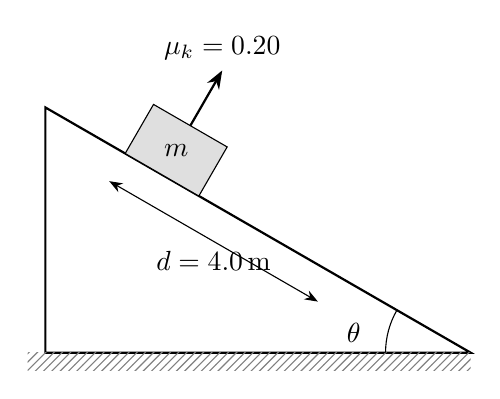
\begin{tikzpicture}[>=Stealth, scale=0.9]
  % incline: A top left, B bottom right, C corner below A
  \coordinate (A) at (0,3.46);
  \coordinate (B) at (6,0);
  \coordinate (C) at (0,0);
  \draw[thick] (A) -- (B) -- (C) -- cycle;
  \fill[pattern=north east lines, pattern color=gray] (-0.25,-0.25) rectangle (6,0);
  % block, sitting on the incline (coordinate system rotated by -30 degrees at A)
  \begin{scope}[shift={(A)}, rotate=-30]
    \draw[fill=gray!25] (1.3,0) rectangle (2.5,0.8) node[midway] {$m$};
    \draw[<->] (1.3,-0.45) -- (4.7,-0.45) node[midway, below] {$d = \qty{4.0}{m}$};
    \draw[->, thick] (1.9,0.8) -- (1.9,1.7) node[above] {$\mu_k = 0.20$};
  \end{scope}
  \draw (4.8,0) arc[start angle=180, end angle=150, radius=1.2];
  \node at (4.35,0.28) {$\theta$};
\end{tikzpicture}
\end{center}

\begin{enumerate}
  \item Draw the free-body diagram of the block and write down Newton's second law along the incline.
        \pts{2}
  \item Find the acceleration of the block down the incline. \pts{3}
  \item What is the speed of the block after it has slid a distance $d = \qty{4.0}{m}$? \pts{3}
  \item What is the smallest coefficient of static friction $\mu_s$ for which the block would stay at rest?
        \pts{2}
\end{enumerate}

% ---- Exercise 3 -----------------------------------------------------------------------
\exercise{3}{Energy and a spring}{8}
A block of mass $m = \qty{0.40}{kg}$ slides from rest from a height $h = \qty{0.60}{m}$ down a
frictionless ramp onto a horizontal track. At the end of the track it hits a spring with spring constant
$k = \qty{250}{N/m}$ that is fixed to a wall.

\begin{center}
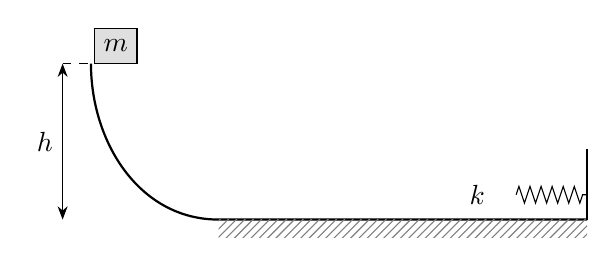
\begin{tikzpicture}[>=Stealth, scale=0.9]
  \draw[thick] (0,2.2) to[out=-90, in=180] (1.8,0) -- (7,0);
  \fill[pattern=north east lines, pattern color=gray] (1.8,-0.25) rectangle (7,0);
  \draw[thick] (7,0) -- (7,1);
  \draw[decorate, decoration={zigzag, segment length=4, amplitude=3}] (6.0,0.35) -- (7,0.35);
  \draw[fill=gray!25] (0.05,2.2) rectangle (0.65,2.7) node[midway] {$m$};
  \draw[<->] (-0.4,0) -- (-0.4,2.2) node[midway, left] {$h$};
  \draw[dashed] (-0.4,2.2) -- (0.05,2.2);
  \node at (5.45,0.35) {$k$};
\end{tikzpicture}
\end{center}

\begin{enumerate}
  \item What is the speed of the block when it reaches the horizontal track? \pts{2}
  \item The whole track is frictionless. By how much is the spring compressed at most? \pts{3}
  \item Now a rough stretch of length \qty{1.0}{m} with $\mu_k = 0.10$ lies between the ramp and the
        spring. By how much is the spring compressed at most in this case? \pts{3}
\end{enumerate}

% ---- Exercise 4 -----------------------------------------------------------------------
\exercise{4}{One-dimensional collision}{8}
On a frictionless air track, cart A ($m_A = \qty{2.0}{kg}$) moves at $v_A = \qty{3.0}{m/s}$ and hits
cart B ($m_B = \qty{1.0}{kg}$), which is at rest.
\begin{enumerate}
  \item The carts stick together (perfectly inelastic collision). Find their common velocity and the
        kinetic energy lost in the collision. \pts{3}
  \item The collision is perfectly elastic. Find the velocities of both carts afterwards. \pts{3}
  \item Explain in one or two sentences why momentum is conserved in both cases, but kinetic energy only
        in case b). \pts{2}
\end{enumerate}

\end{document}
